\chapter{Anwendunge der Galoistheorie}
\section{Endliche Körper}
\begin{Lemma}
	Sei \(K\) ein beliebiger Körper der Charakteristik \(p>0\). Die Abbildung 
	\(\phi\colon K\to K,\ \phi(x)=x^p\) ist ein Ringhomomorphismus.
	Wenn \(K\) endlich ist, dann ist
	\(\phi\) bijektiv.
\end{Lemma}
\begin{proof}
	Es ist \[\phi(x+y)=\sum_{i=0}^p\binom{p}{i}x^iy^{p-i}=y^p+x^p=\phi(x)+\phi(y)\]
	\(\phi\) ist immer injektiv. Wenn \(K\) endlich ist, dann automatisch bijektiv.
\end{proof}
\begin{Def}
	Sei \(q=p^r\) und \(\FF_q\) ein Zerfällungskörper von \(x^q-x\) über \(\FF_p.\)
\end{Def}
\begin{Satz} Sei \(q=p^r\) für eine Primzahl \(p\).
	\(\FF_q\) ist ein endlicher Körper mit \(q\) Elementen und jeder endlich Körper ist isomorph zu \(\FF_q\) für ein \(q=p^r\) wobei \(p=\chara K\).
\end{Satz}
\begin{proof}
	Sei \(K\) irgendein endlicher Körper der Charakteristik \(p>0\) und \(b\in K\). Es ist \((X^q-X)(b)=0\iff \phi^r(b)=b\). Dann ist \(\set{x\in K}{ \phi^r(x)=x}\) ein Teilkörper von \(K\).
	In \(\FF_q[X]\) zerfällt \(X^q-X\) in Linearfaktoren. Die Ableitung ist \((X^q-X)'=-1\) was teilerfremd ist zu \(X^q-X\). Also ist \(X^q-X\) separable. Also hat \(X^q-X\) \(q\)-viele verschiedene Nullstellen, die einen Teilkörper \(L\subseteq \FF_q\) bilden. Somit \(\FF_q=L\) und \(|\FF_q|=q\).
	Sei \(K\) ein endlicher Körper der Charakteristik \(p\). Dann ist \([K:\FF_p]=r<\infty\) und damit \(|K|=p^r=q\).
	Für \(a\in K\) gilt \(a^q=a\). Denn wenn \(a=0\) dann ist das richtig und wenn \(a\neq 0\) dann ist \(a\in K^*\) und \(|K^*|=q-1\). Nach \nameref{Kor:Lagrange2} gilt \(a^{q-1}=1\) also \(a^q=a\) für alle \(a\in K\). Das heißt \(x^q-x\) zerfällt in \(K[X]\) und somit gibt es Homomorphismus \(\FF_q\to K\) mit \(|\FF_q|=q=|K|\) also ist \(\FF_q\cong K\).
\end{proof}
\begin{Satz}
	Sei \(K\) ein beliebiger Körper und \(G\subseteq K^*\) eine endliche Untergruppe. Dann ist \(G\) zyklisch.
\end{Satz}
\begin{proof}
	Sei \(n=|G|\). Der Struktursatz für endlich abelsche Gruppen impliziert 
	\[G\cong \ZZ/m_1\ZZ\times \dots\times \ZZ/m_r\ZZ\] mit \(m_1|m_2|\dots| m_r\) und \(n=\prod_{i=1}^rm_i\).
	Für jedes \(a\in G\) gilt \(a^{m_r}=1\). Sei also \(f=X^{m_r}-1\). Jedes \(a\in G\) ist Nullstelle von \(f\) und \(f\) hat höchstens \(m_r\) verschiedene Nullstellen. Somit ist \(n=m_r\) und \(G\cong \ZZ/m_r\ZZ\) zyklisch.
	
\end{proof}
\begin{Kor}
	Wenn \(K\) ein endlicher Körper ist, dann ist \(K^*\) zyklisch mit \(K^*\cong \ZZ/(q-1)\ZZ\)
\end{Kor}
\begin{Bsp}
	Sei \(K=\CC\) und \(G=\set{z\in\CC}{ z^n=1}=\mu_n(\CC)\). Dann ist \(G\) zyklisch. \(x^n-1\) ist separable da die Ableitung nicht \(0\) ist. Somit ist \(G\cong \ZZ/n\ZZ\) \(G=\set{e^{2\pi i k/n}}{ 0\leq k\leq n-1}\) erzeugt von \(e^{2\pi i/n}\). 
	Es gilt: \(e^{2\pi i k/n}\) erzeugt \(\mu_n(\CC)\) genau dann wenn \(\ggT(k,n)=1\).
\end{Bsp}
\begin{Def}
	Sei \(f\in K[X]\) ein separables Polynom und \(L/K\) ein Zerfallskörper von \(f\). Die Galoisgruppe von \(f\) ist \(\Gal(L/K)\)
\end{Def}
\begin{Bem}
	Sei \(N\) die Menge der Nullstellen von \(f\) in \(L\).
	Haben injektiven Gruppenhomomorphismus \(\Gal(L/K)\to S(N)\cong S_n,\ \sigma\mapsto \sigma|_N\) wobei \(n=\deg(f)=|N|\). Das zeigt
\end{Bem}
\begin{Satz}
	Wenn \(L/K\) Zerfällungskörper eine separablen Polynoms \(f\) von Grad \(n\) ist, dann \(\Gal(L/K)\to S_n\) injektiv.
\end{Satz}
\begin{Def}[Diskriminante]
	Sei \(f\in K[X]\) ein normiertes Polynom, \[f=\prod_{i=1}^n(X-\alpha_j)\] in \(\bar K[X]\) und \(n=\deg(f)\). Sei 
	\[\delta=\prod_{\stackrel{i,j\in\Set{1,\dots,n} }{i<j}}(\alpha_i-\alpha_j)\in\bar K.\]
	Dann ist \(\Delta=\delta^2\in\bar K\) die Diskriminante von \(f\)
\end{Def}
\begin{Lemma}
	Es ist \(\Delta\in K\) und es gilt  \[\Delta\neq 0\iff f \text{ ist separable.}\]
\end{Lemma}
\begin{proof}
	Sei \(\Delta\neq 0\) und \(L/K\) Zerfällungskörper von \(f\).
	Dann ist \(L/K\) Galoisch und für \(\sigma\in G=\Gal(L/K)\) gilt
	\[\sigma(a_i)-\sigma(\alpha_j)=\alpha_{i'}-\alpha_{j'}=-(\alpha_{j'}-\alpha_{i'})\] 
	und einer der letzten beiden Terme taucht als Faktor in \(\delta\) auf. Also ist \(\sigma(\delta)=\pm \delta\) und damit \(\sigma(\Delta)=\Delta\). Also gilt \(\Delta\in L^G=K\).
\end{proof}
\begin{Bem}
	Wenn \(f\) separablel, dann ist für \(\sigma\in\Gal(L/K)\) \[\sigma(\delta)=\sign(\sigma)\delta\] wobei wir \(\sigma\) als Element in \(S_n\) auffassen.
\end{Bem}
\begin{Bem}
	sei \(f\in K[X]\) und \(n=\deg(f)\).
	\begin{enumerate}
		\item Sei \(n=2\) und \(f=X^2+pX+q=(X-\alpha_1)(X-\alpha_2)=X^2-(\alpha_1+\alpha_2)X+\alpha_1\alpha_2\)
		und \[\Delta=(\alpha_1-\alpha_2)^2=(\alpha_1+\alpha_2)^2-4\alpha_1\alpha_2=p^2-4q\]
		\item Sei \(n=3\) und \(\chara (K)\not\in\Set{2,3}\) und \(f=X^3+a_2X^2+a_1X+a_0\). Für \(Y=X+\frac{1}{3}a_2\) erhalten wir können wir \(X\) ersetzen und behalten die gleiche Diskrimminante. Wir bekommen
		\begin{align*}
			f&=(Y-\frac{1}{3}a_2)^3+a_2(Y-\frac 13 a_2)^2+a_1(Y-\frac 1 3a_2)+a_0\\
			&=Y^3+aY+b
		\end{align*} für irgendwelche \(a,b\in K\). Sei also \(f=X^3+aX+b\). Eine ähnliche 
		Rechnung wie für \(n=2\) ergibt \(\Delta=-4a^3-27b^2\)
	\end{enumerate}
\end{Bem}
\begin{Satz}
	Sei \(\chara (K)\not\in\Set{2,3}\) und \(f=X^3+aX+b\in K[X]\) irreduzibel. Dann ist ein Zerfällungskörper \(L/K\) von \(f\) Galoisch. Es ist \(\Gal(L/K)\subseteq S_3\).
	\begin{enumerate}
		\item \(\Delta\) ist Quadrat in \(K\implies G=A_3\cong\ZZ/3\ZZ\)
		\item \(\Delta\) kein Quadrat in \(K\implies G=S_3\)
	\end{enumerate}
\end{Satz}
\begin{proof}
	Da \(f\) irreduzibel gilt für eine Nullstelle \(\alpha\) von \(f\) dass \([K(\alpha):K]=3\) ist. Also ist \([L:K]\in\Set{3,6}\).
	Die einzigen Untergruppen von \(S_3\) mit 3 bzw. 6 Elementen sind \(A_3\) bzw \(S_3\)
	\begin{align*}
		G=A_3&\iff G=\ker(\sign\colon S_3\to\Set{\pm 1})\\
		&\iff \forall\sigma\in G: \sign(\sigma)=1\\
		&\iff \forall \sigma\in G\colon \sigma(\delta)=\delta\\
		&\iff \delta\in L^G=K\\
		&\iff \Delta \text{ ist Quadrat in K}
	\end{align*}
\end{proof}
\begin{Bsp}
	Sei \(f=X^3-a\) wobei \(a\)  keine dritte Potenz in \(K=\QQ\) ist.
	\(f\) hat keine Nullstelle also ist \(f\) irreduzibel. \(\Delta=-27a^2\) ist kein Quadrat in \(\QQ\). Also ist \(\Gal(L/K)=S_3\)
\end{Bsp}
\begin{Lemma}\label{Lem:RatNst}
	Sei \(R\) faktoriell und \(g,h\in K[X]\) normiert und sei \(K=\Quot(R)\). Wenn \(g\cdot h\in R[X]\) dann ist \(g,h\in R[X]\).
\end{Lemma}
\begin{proof}
	Es ist \(g/c(g), h/c(h)\in R[X]\). Also sind \(1/c(g),1/c(h)\in R\) da \(g,h\) normiert.
	Es ist \(1=c(gh)=c(g)c(h)\) also ist \(1/c(g),1/c(h)\in R^*\) also ist \(c(g),c(h)\in R^*\) also ist \(h,g\in R[X]\).
\end{proof}
\begin{Kor}
	Wenn \(f\in\ZZ[X]\) normiert ist und \(a\in\QQ\) eine Nullstelle von \(f\), dann ist \(f=(X-a)\cdot g\), wobei \(g\) normiert ist. Dann ist \(a\in\ZZ\) und \(g\in\ZZ\).
\end{Kor}
\begin{Bsp}
	\(X^3-3x+1\) mögliche Nullstellen in \(\QQ\) sind Teiler von \(1\) in \(\ZZ\). Das sind aber keine Nullstellen, also ist \(f\) irreduzibel in \(\QQ[X]\).
	\(\Delta=-4(-3)^3-27\cdot 1^2=3^4\) ist Quadrat, also \(\Gal(L/K)=A_3\)
\end{Bsp}
\section{Kreisteilungskörper}
\begin{Def}
	Sei \(K\) ein Körper und \(\mu_n(K)=\set{x\in K}{ x^n=1}\) Gruppe der \(n\)-ten Einheitswurzeln in \(K\).
\end{Def}
\begin{Satz}
	Sei \(\chara (K) \not\mid n\). Dann ist \(\mu_n(\bar K)\) zyklisch von Ordnung \(n\).
\end{Satz}
\begin{proof}
	\(f=X^n-1\) und \(f'=nX^{n-1}\neq 0\). Einzige Nullstelle von \(f'\) ist \(x=0\) aber \(f(0)\neq 0\). Somit ist \(ggT(f,f')=1\) und damit \(f\) separabel.
\end{proof}
\begin{Def}
	Sei \(\chara (K)\not\mid n\). Ein \(\zeta\in\mu_n(K)\) heißt primitive \(n\)-te Einheitswurzel, wenn \(\zeta\) die Gruppe \(\mu_n(\bar K)\) erzeugt. Sei \(K(\zeta_n)=K(\mu_n(\bar K))\) der Zerfällungskörper von \(x^n-1\). \(K(\zeta_n)\) heißt der \(n\)-te Kreisteilungskörper über \(K\).
\end{Def}
\begin{Lemma}\label{Lem:MorGSn}
	Sei \(G\) eine zyklische Gruppe mit \(|G|=n\). Dann ist \(\End(G)\cong \ZZ/n\ZZ\) als Ring und \(\Aut(G)\cong (\ZZ/n\ZZ)^*\) als Gruppe.
\end{Lemma}
\begin{proof}
	Wähle Isomorphismus \(\psi\colon \ZZ/n\ZZ\to G\) Wenn \(f\colon G\to G\) Endomorphismus ist, dann ist \(\psi^{-1}f\psi\) ein Endomorphismus von \(\ZZ/n\ZZ\).
	somit \(End(G)\cong End(\ZZ/n\ZZ)\cong \ZZ/n\ZZ\) denn Endomorphismen eindeutig bestimmt durch \(f(1)=a\).
\end{proof}
\begin{Def}
	Die Anzahl der zu \(n\) teilerfremden Zahlen in \(\Set{0,1,\dots,n-1}\) ist \[\varphi(n)=\abs{(\ZZ/n\ZZ)^*}.\] Die Funktion \(\varphi\) heißt Eulersche \(\varphi\)-Funktion
\end{Def}
\begin{Lemma} Es gilt
	\begin{enumerate}
		\item  \(\ggT(n,m)=1\implies \varphi(nm)=\varphi(n)\varphi(m)\)
		\item \(\varphi(\kgV(n,m))\varphi(\ggT(n,m))=\varphi(n)\varphi(m)\)
		\item Wenn \(n=\prod_{i=1}^rp_i^{e_i}\) wobei \(p_i\) paarweise verschiedene Primzahlen, dann ist 
		\[\varphi(n)=\prod_{i=1}^n\varphi(p_i^{e_i})=\prod_{i=1}^n(p_i-1)p_i^{e_i-1}\]
	\end{enumerate}
\end{Lemma}
\begin{proof}
	Nach Chinsesischem Restzatz ist \(\ZZ/nm\ZZ\cong \ZZ/n\ZZ\times \ZZ/m\ZZ\) also gilt die erste Aussage. Die zweite Aussage folgt aus der ersten.
	Für die dritte reicht \(\varphi(p^e)=p^{e-1}(p-1)\) für eine Primzahl \(p\).
	Nicht-Einheiten in \(\ZZ/p^e\ZZ\) sind \(0,p,2p,\dots,(p^{e-1}-1)p\), das sind also \(p^{e-1}\) viele. Somit \(|(\ZZ/p^e\ZZ)^*|=p^e-p^{e-1}\)
\end{proof}
\begin{Satz}
	Sei \(L=K(\zeta_n)/K\). Die Abbildung 
	\[\psi\colon\Gal(L/K)\to\Aut\mu_n(\bar K),\; \sigma\mapsto \sigma|_{\mu_n(L)}\] ist ein injektiver Gruppenhomomorphismus.
\end{Satz}
\begin{proof}
	\(\psi\) ist injektiv, da \(L/K\) von \(\mu_n(L)\) erzeugt ist.
\end{proof}
\begin{Kor}\label{Kor:ChiGal}
	Sei \[\phi\colon(\ZZ/n\ZZ)^*\to Aut(\mu_n(\bar K)),\ a\mapsto (\mu_n(\bar K)\to\mu_n(\bar K),\ \zeta\mapsto \zeta^a)\] der Isomorphismus aus \Cref{Lem:MorGSn}.
	Dann ist \[\chi=\phi^{-1}\psi\colon G\to (\ZZ/n\ZZ)^* \] gegeben durch \[\zeta^{\chi(\sigma)}=\zeta^{\phi^{-1}(\sigma|_{\mu_n(\bar K)})}=\sigma(\zeta).\]
	Insbesondere ist \(\chi\) injektiv und \(\sigma(\zeta_n)=\zeta_n^{\chi(\sigma)}\) und dadurch \(\chi(\sigma)\) schon bestimmt.
\end{Kor}
\begin{Kor}
	\(\Gal(K(\zeta_n)/K)\) ist eine abelsche Gruppe.
\end{Kor}
\begin{Bsp}
	\(K=\RR\) and \(n\geq 3\). Dann ist \(\mu_n(\CC)\subsetneq\RR\) und somit \(K(\mu_n(\CC))=\CC\).
	\(\Gal(\CC/\RR)=\Set{\id,\sigma}\) wobei \(\sigma\) die komplexe Konjugation ist. Es ist \(\chi(\sigma)=-1\) denn
	für \(\zeta\in\mu_n(\CC)\) ist \(\sigma(\zeta)=\bar\zeta=\zeta^{-1}\)
\end{Bsp}
\begin{Satz}
	Sei \(q=p^r\) für eine Primzahl \(p\) und \(L/\FF_q\) eine endliche Galoiserweiterung. Dann ist \(G=\Gal(L/\FF_q)\) von \(\phi_q\) erzeugt, wobei \(\phi_q(x)=x^q\).
\end{Satz}
\begin{proof}
	\(\FF_q\) ist Zerfällungskörper von \(x^q-x\) über \(\FF_p\) und
	\(\FF_q=\set{x\in L}{ \phi_q(x)=x}\). Somit ist \(\phi_q\in G\).
	Für \(H=\langle \phi_q\rangle\subseteq G\) ist 
	dann \(L^H=\FF_q=L^G\) also ist \(H=G\).
\end{proof}
\begin{Kor}
	Sei \(q=p^r\) und \(n\in\NN\) mit \(p\not\mid n\). Sei \(L=\FF_q(\zeta_n)\) wobei \(\zeta_n\in\bar \FF_q\) primitive \(n\)-te Einheitswurzel.
	Sei \(\chi\colon \Gal(L/\FF_q)\to (\ZZ/n\ZZ)^*, \phi_q\mapsto k=\chi(\phi_q)\) wie in \Cref{Kor:ChiGal}. Dann ist
	\[|\Gal(L/\FF_q)|=\ord(\phi_q)=\ord(\chi(\phi_q))=\ord(q\in(\ZZ/n\ZZ)^*)\]
\end{Kor}
\begin{Bsp}
	Sei \(n=12\) und \(p=7\). Es ist \(7^2=49 =48+1\) also ist die Ordnung von \(7\) gleich 2.
	Also \([\FF_7(\zeta_{12}):\FF_7]=|\Gal(..)]=2\) und somit \(\FF_7(\zeta_{12})=\FF_{49}\)
\end{Bsp}
\begin{Satz}
	Der Homomorphismus \(\chi\colon\Gal(\QQ(\zeta_n/\QQ)\to(\ZZ/n\ZZ)^*\) aus \Cref{Kor:ChiGal} ist bijektiv, das heißt \([\QQ(\zeta_n)\colon \QQ]=\varphi(n)\).
\end{Satz}
\begin{proof}
	Sei \(\zeta_n\in\bar\QQ\) eine primitive \(n\)-te Einheitswurzel und \(f\in\QQ[x]\) das Minimalpolynom von \(\zeta_n\).
	Wir zeigen, dass jede andere primitive \(n\)-te Einheitswurzel auch Nullstelle von
	\(f\) ist. Dann ist \(
	\deg(f)\) die Anzahl der primitiven \(n\)-ten Einheitswurzeln und somit 
	\([\QQ(\zeta_n):\QQ]=\varphi(n)\).
	Denn wenn \(m\) eine Einheit ist in \(\ZZ/n\ZZ\) dann ist \(\zeta_n^m\) eine primitve Einheitswurzel.
	Ohne Einschärnkung \(m=p\) prim.
	Sei also \(p\not\mid n\) und \(g\) Minimalpolynom von \(\zeta_n^p\). Angenommen \(f\neq g\).
	Es ist \(\zeta_n^{pn}-1=0\) also teilt \(f\mid X^n-1,\ g\mid X^n-1\) also \(f\cdot g\mid X^n-1\). Nach \Cref{Lem:RatNst} folgt \(f,g\in\ZZ[X]\) und außerdem ist \(\zeta_n\) eine Nullstelle von \(g(X^p)\) also \(f\mid g(X^p)\) und \(g(X^P)=f\cdot h\) für ein \(h\in \ZZ[X]\).
	In \(\FF_p[X]\) gilt \(f\mid g(X^p)=g(X)^p\) also sind \(f\) und \(g\) nicht teilerfremd in \(\FF_p[X]\). Da aber \(f\cdot g\mid X^n-1\) kommt ein irreduzibler Faktor von \(X^n-1\) doppelt vor, was ein Widerspruch dazu ist, dass \(X^n-1\) separabel ist über \(\FF_p\).
	Also ist \(f=g\)
\end{proof}
\begin{Kor}
	Für \(n,m\in\ZZ\) mit \(\ggT(n,m)=d\) und \(\kgV(n,m)=k\) gilt \[\QQ(\zeta_n)\cap \QQ(\zeta_m)=\QQ(\zeta_d)\] und \[\QQ(\zeta_n)\QQ(\zeta_m)=\QQ(\zeta_k)\]
\end{Kor}
\begin{proof}
	Es ist \(\QQ(\zeta_k)\supseteq\QQ(\zeta_n)\QQ(\zeta_m)\).
	Sei \(\zeta_n\) eine primitive \(n\)-te Einheitswurzel und \(\zeta_m\) primitive \(m\)-te Einehitswurzel und sei \(d=an+bm\) für \(a,b\in\ZZ\).
	Dann ist \(\xi=\zeta_n^b\zeta_m^a\) primitive \(k\)-te Einheitswurzel, denn \(\xi^k=1\) und wenn \(\xi^s=1\)ist, dann ist \(\zeta_n^{sb}=\zeta_m^{-sa}\) woraus \(n\mid sbm\) und somit \(n\mid sd\) folgt. Also \(n/d\mid s\). Analog \(m/d\mid s\) also folgt zusammen \(k\mid s\). Also gilt \[\QQ(\zeta_k)=\QQ(\zeta_n)\QQ(\zeta_m).\] Außerdem gilt
	\(\QQ(\zeta_d)\subseteq \QQ(\zeta_n)\cap\QQ(\zeta_m)\).
	Für \(M=\QQ(\zeta_n)\), \(K'=\QQ(\zeta_n)\), \(K=\QQ\) und \(M'=MK'\) gilt nach \Cref{Satz:Translat}
	\begin{align*}
		\varphi(k)\varphi(d)&=\varphi(n)\varphi(m)\\
		&=[M:K]\cdot [K':K]\\
		&=[M':K][K'\cap M:K]\\
		&=\varphi(k)[K'\cap M:K]
	\end{align*}
	Also \(K'\cap M=\QQ(\zeta_d)\)
\end{proof}
\begin{Def}
	Sei \(n\in\NN\). Das \(n\)-te Kreisteilungspolynom ist \[\phi_n=\prod_{\stackrel{\zeta\in\mu_n(\CC)}{\text{ primitiv}}}(X-\zeta)=\prod_{k\in(\ZZ/n\ZZ)^*}(X-\zeta_n^k)\in\CC[X]\] für \(\zeta_n=e^{2\pi i/n}\)
\end{Def}
\begin{Lemma}
	Es gilt    \[X^n-1=\prod_{d\mid n}\phi_d\]
\end{Lemma}
\begin{proof}
	Es ist \[X^n-1=\prod_{\zeta\in\mu_n(\CC)}(X-\zeta)\] und jedes \(\zeta\) ist eine primitive \(d\)-te Einheitswurzel für \(d=\ord(\zeta)\) und jede primitive \(d\)-te Einheitswurzel für \(d\mid n\) ist ein Element von \(\mu_n(\CC)\).
	Dann impliziert \[\mu_n(\CC)=\coprod_{d\mid n}\Set{\zeta_d \text{ primitive \(d\)-te Einheitswurzel}}\] die Aussage.
\end{proof}
\begin{Lemma}
	Es ist \(\phi_d\in\ZZ[X]\) und \(\phi_d\) ist das Minimalpolynom von \(\zeta_d\) über \(\QQ\).
\end{Lemma}
\begin{proof}
	Klar
\end{proof}
\begin{Bem}
	Für \(n=p\) prim gilt \(\phi_p=(X^p-1)/(X-1)=\sum\limits_{k=0}^{p-1}X^k\)
\end{Bem}
\begin{Bsp}
	\(\QQ(\zeta_9)/\QQ\) hat Galoisgruppe \((\ZZ/9\ZZ)^*\) mit \(\phi(9)=6\) Elementen. Der \nameref[Satz:StuktEndlAb] liefert \[G\cong \ZZ/2\ZZ\times \ZZ/3\ZZ\] und das hat die vier Untergruppen \(\Set{0},\ZZ/2\ZZ\times\Set{0}, \Set{0}\times\ZZ/3\ZZ\).
	Das entspricht den Untergruppen \(\Set{1}, \langle-1\rangle, \langle 4\rangle,G\).
	Es ist \(\chi(\sigma)=-1\) für die komplexe Konjugation \(\sigma\colon\CC\to\CC\). Also ist für \(L=\QQ(\zeta_9)\)
	\[L^{\langle -1\rangle}=L\cap \CC^{\langle \sigma\rangle}=L\cap\RR=\QQ(\zeta_9+\zeta_9^{-1})\]
	Wobei die letzte Gleichung gilt, da für \(b=\zeta_9+\zeta_9^{-1}\)
	\[b\zeta_9=\zeta_9^2+1\] also ist \(\zeta_9^2-b\zeta+1=0\) und somit \([\QQ(\zeta_9):\QQ(b)]\leq 2\).
	Da \(\QQ(\zeta_3)\subseteq \QQ(\zeta_9)\) und \([\QQ(\zeta_3):\QQ]=2\) folgt \(L^{\langle 4\rangle}=\QQ(\zeta_3)\).
\end{Bsp}
\section{Konstruktion mit Zirkel und Lineal}
Starte mit einer Menge von Punkten in \(\RR^2=\CC\)
Erlaubte Konstruktionen: Geraden durch 2 Verschiedene Punkte die gegeben sind und Kreise durch 2 Punkte, einer davon der Mittelpunkt, und Schnittpunkte von 2 Objekten dieser Art.
\begin{Bsp}
	Man kann gleichseitige Dreiecke konstruieren.
	\begin{center}\begin{tikzpicture}
			% Define coordinates
			\coordinate (P) at (0,0);
			\coordinate (Q) at (2,0);
			
			% Draw a circle and name its path
			\draw[name path=mycircleP] (P) circle (2cm);
			\draw[name path=mycircleQ] (Q) circle (2cm);
			
			% Draw a line and name its path
			\draw[name path=myline] (P) -- (Q);
			
			% Find the intersections and name them
			\path[name intersections={of=mycircleP and mycircleQ, by={R, S}}];
			
			% Mark the intersection points (optional)
			\fill[red] (R) circle (2pt) node[above right] {\(R\)};
			%\fill[red] (S) circle (2pt) node[below right] {\(P_2\)};
			
			% You can also draw a triangle using its vertices
			\draw[blue, thick] (P) -- (R) -- (Q) -- cycle;
	\end{tikzpicture}\end{center}
\end{Bsp}
\begin{Bem}
	Klassische Probleme sind
	\begin{enumerate}
		\item Winkeldreiteilung: Wenn \(P, R_1,R_2,R_3\) gegeben sind, suche \(R_3\) sodass \(3\alpha=\beta\).
		\begin{center}\begin{tikzpicture}
				\coordinate (P) at (0,0);
				\coordinate (R_1) at (4*0.5,4*0.866);
				\coordinate (R_2) at (4*1,0);
				\coordinate (R_3) at (4*0.766,4*0.642);
				\draw  (P) -- (R_1);
				\draw (P) -- (R_2);
				\draw (P) -- (R_3);
				
				\fill[black] (P) circle (2pt) node[above left] {\(P\)};
				\fill[black] (R_1) circle (2pt) node[above right] {\(R_1\)};
				\fill[black] (R_2) circle (2pt) node[above right] {\(R_2\)};
				\fill[black] (R_3) circle (2pt) node[above right] {\(R_3\)};
				% Calculate and draw the angle
				% The "angles" library makes this easy
				% The syntax is: pic [draw, angle radius, "label", angle eccentricity] {angle = B--O--A};
				% 'angle radius' controls the size of the arc
				% 'angle eccentricity' controls the label's distance from the arc
				\pic [draw, red, "\(\alpha\)", angle radius=0.8cm, angle eccentricity=1.3] {angle = R_3--P--R_1};
				
				\pic [draw, blue, "\(\beta\)", angle radius=1.5cm, angle eccentricity=1.3] {angle = R_2--P--R_1};
				
				% Alternative way to label an angle, for more control:
				% 1. Create an invisible path for the angle
				% \path (A) -- (O) -- (B) coordinate [pos=0.5] (angle_center_OAB); % Center of the angle arc
				% 2. Draw the arc
				% \draw[red] (O) +(\((A)-(O)\)!0.5cm!90:(B)-(O)) arc [start angle={atan2((A)-(O) split at y, (A)-(O) split at x)}, end angle={atan2((B)-(O) split at y, (B)-(O) split at x)}, radius=0.5cm];
				% 3. Place the label
				% \node[red] at (angle_center_OAB) [label=45:\(\alpha\)] {}; % Adjust '45' for angle of label placement
				
		\end{tikzpicture}\end{center}
		\item Würfeldoppelung: Gegeben \(P,Q\) suche \(Q'\) sodass \(|PQ'|^3=2|PQ|^3\).
		\item Quadratur des Kreises: Gegeben \(P,Q\) suche \(Q'\) sodass \(|PQ|^2=\pi |PQ|^2\).
		\item Kubatur der Kugel: Suche \(Q'\) sodass Würfel mit Kante \(PQ'\) das gleiche Volumen hat wir Kugel mit Radius \(PQ\).
		\item Konstruktion des regulären \(n\)-Ecks mit 2 gegebenen benachbarten Ecken.
	\end{enumerate}
\end{Bem}
\begin{Def}
	Für \(z,w\in\CC\) sei \[\ell(z,w)=\set{z+\lambda(w-z)}{ \lambda\in\RR}\] die Gerade durch \(z,w\) und \[k(z,w)=\set{w'\in\CC}{ |z-w|=|z-w|'}=\set{z+\lambda (w-z)}{ \lambda\in\CC, |\lambda|=1}\] der Kreis mit Mittelpunkt \(z\) durch \(w\).
\end{Def}
\begin{Def}
	Für \(M\subseteq \CC\) sei \(K(M)\subseteq \CC\) die kleinste Menge sodass
	\begin{enumerate}
		\item \(M\subseteq K(M)\)
		\item Wenn \(z,w,z',w'\in K(M)\) mit \(z\neq w\) und \(z'\neq w'\) dann 
		\[\ell(z,w)\cap \ell(z',w')\subseteq K(M)\]
		\[\ell(z,w)\cap k(z',w')\subseteq K(M)\]
		\[k(z,w)\cap k(z',w')\subseteq K(M)\] falls die Schnitte jeweils endlich sind.
	\end{enumerate}
	\(K(M)\) ist die Menge aller Elemente von \(\CC\) die durch endlich viele Schnitte in \(M\) wie oben gewonnen werde können. Wir nennen \(K(M)\) die Menge der aus \(M\) konstruierbaren Zahlen.
\end{Def}
\begin{Bem}
	Wenn \(M\neq \emptyset\) oder \(|M|=1\) dann ist \(K(M)=M\).
	Sei \(|M|\geq 2\). Ohne Einschränkung \(0,1\in M\).
	Es gilt
	\begin{enumerate}
		\item \(\ZZ\subseteq K(0,1)\)
		\begin{center}\begin{tikzpicture}
				\draw (-2,0) -- (3,0);
				\coordinate (P) at (-1,0);
				\coordinate (R_1) at (0,0);
				\coordinate (R_2) at (1,0);
				\coordinate (R_3) at (2,0);
				
				\pic [draw, black, "\( \)", angle radius=1cm, angle eccentricity=1] {angle = R_2--R_1--P};
				\pic [draw, black, "\( \)", angle radius=1cm, angle eccentricity=1] {angle = R_3--R_2--R_1};
				\fill[black] (P) circle (2pt) node[below ] {\(-1\)};
				\fill[black] (R_1) circle (2pt) node[below ] {\(0\)};
				\fill[black] (R_2) circle (2pt) node[below ] {\(1\)};
				\fill[black] (R_3) circle (2pt) node[below ] {\(2\)};
		\end{tikzpicture}\end{center}
		\item Man kann Orthogonalen zu einer Geraden durch einen Punkt konstruieren. Seien \(P,Q\) und \(\bar{PQ}\) gegeben. Sei \(R'\) nicht auf \(\bar{PQ}\). Bilde den roten Kreis und danach den blauen. Das gibt Schnittpunkt \(R''\) Die grüne Gerade ist Orthogonale
		\begin{center}\begin{tikzpicture}
				\coordinate (P) at (-2,0);
				\coordinate (R') at (1,1);
				\coordinate (R'') at (1,-1);
				
				\draw[name path=myline] (-3,0) -- (5,0);
				\draw[name path=mycircleP, red] (R') circle (2cm);
				\path[name intersections={of=mycircleP and myline, by={Q, Q'}}];
				\draw[name path=kreis, blue] (Q) circle (2cm);
				\fill[black] (P) circle (2pt) node[below ] {\(P\)};
				\fill[black] (R') circle (2pt) node[above right] {\(R'\)};
				\fill[black] (Q) circle (2pt) node[below left] {\(Q\)};
				\fill[red] (Q') circle (2pt) node[below right] {\(Q'\)};
				\fill[purple] (R'') circle (2pt) node[below right] {\(R''\)};
				\draw[green] (R') -- (R'');
				
				
				
		\end{tikzpicture}\end{center}
		\item Parallele zu Geraden durch Punkt R
		\begin{center}\begin{tikzpicture}
				\draw (-1,0) -- (1,0);
				\draw[red] (-1,1) -- (1,1);
				\coordinate (R) at (0,1);
				\fill[black] (R) circle (2pt) node[above] {\(R\)};
				
		\end{tikzpicture}\end{center} Verfahren: Bestimme Orthogonale durch \(R\). Dann 
		konstruire gleichseitiges Dreieck wo \(R\) der Mittelpunkt einer Seite ist. Das gibt Parallele.
		\item Veschiebung von Vektoren. Seien \(P,Q,R\) gegeben. Suche \(R+(Q-P)\). Klar, Konstruiere Parallele, Verbinde Punkte und konstruiere parallele.
	\end{enumerate}
\end{Bem}
\begin{Lemma}
	Sei \(0,1\in M\) und \(a\in\CC\). Es ist äquivalent:
	\begin{enumerate}
		\item \(a\in K(M)\)
		\item \(\bar a\in K(M)\)
		\item \(\Re(a),\Im(a)\in K(M)\)
		\item \(|a|, \frac{a}{|a|}\in K(M)\)
	\end{enumerate}
	\begin{center}\begin{tikzpicture}
			\coordinate (P) at (1,0);
			\coordinate (Q)  at (0,1);
			\coordinate (R) at (0,1.5);
			\coordinate (S) at (1.7,0);
			\coordinate (T) at (1.7,1.5);
			\coordinate (O) at (0,0);
			\draw[name path=xAchse] (-1,0) -- (2,0);
			\draw[name path=yAsche] (0,0) -- (0,2);
			\draw[red] (0,0) -- (T);
			\draw[red] (R) -- (T);
			\draw[red] (S) -- (T);
			\pic [draw, red, "\( \)", angle radius=1cm, angle eccentricity=1] {angle = P--O--Q};
			\fill[black] (P) circle (2pt) node[below ] {\(1\)};
			\fill[black] (Q) circle (2pt) node[ left] {\(i\)};
			\fill[black] (R) circle (2pt) node[left] {\(\Im(a)\)};
			\fill[black] (S) circle (2pt) node[below ] {\(\Re(a)\)};
			\fill[black] (T) circle (2pt) node[above right] {\(a\)};
			\fill[black] (0.749,0.661) circle (2pt) node[ right] {\(\frac{a}{|a|}\)};
			
			
			
	\end{tikzpicture}\end{center}
\end{Lemma}
\begin{Lemma}
	Sei \(0,1\in M\). Dann ist \(K(M)\) ein Körper. Insbesondere ist \(\QQ\subseteq K(M)\).
\end{Lemma}
\begin{proof}
	Zeige, dass \(K(M)\) abgeschlossen ist unter Multiplikation und Inverse.
	Für Multiplikation reicht die Multiplikation von reellen Zahlen und von Zahlen mit Betrag 1 (dh. Addition von Winkeln).
	\begin{center}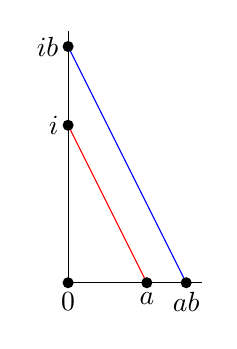
\begin{tikzpicture}
			\coordinate (I) at (0,2);
			\coordinate (A) at (1,0);
			\coordinate (IB) at (0,3);
			\coordinate (AB) at (1.5,0);
			\draw[black] (0,0) -- (0,3.2);
			\draw[black] (0,0) -- (1.7,0);
			\draw[red] (I) -- (A);
			\draw[blue] (IB) -- (AB);
			\fill[black] (I) circle (2pt) node[left] {\(i\)};
			\fill[black] (IB) circle (2pt) node[left] {\(ib\)};
			\fill[black] (A) circle (2pt) node[below] {\(a\)};
			\fill[black] (AB) circle (2pt) node[below] {\(ab\)};
			\fill[black] (0,0) circle (2pt) node[below] {\(0\)};
	\end{tikzpicture}\end{center}
	Addition von Winkeln:
	\begin{center}\begin{tikzpicture}
			\coordinate (N) at (0,0);
			\coordinate (E) at (4,0);
			\coordinate (Z) at (4*0.923,4*0.382);
			\coordinate (W) at (4*0.623,4*0.781);
			\coordinate (W') at (4*0.276,4*0.961);
			\coordinate (yE) at (0,4);
			\draw[name path=xAchse] (0,0) -- (4,0);
			\draw[name path=yAchse] (0,0) -- (0,4);
			\draw[name path=erste]  (0,0) -- (Z);
			\draw[name path=zweite] (0,0) -- (W);
			\draw[name path= dritte] (0,0) -- (W');
			\draw[green] (W) -- (4.053,3.127) node[midway, above] {\(|z-1|\)};
			\pic [draw, black, "\( \)", angle radius=4cm, angle eccentricity=1] {angle = E--N--yE};
			\pic [draw, red, "\(\alpha \)", angle radius=1.8cm, angle eccentricity=0.7] {angle = E--N--Z};
			\pic [draw, blue, "\( \beta\)", angle radius=2.5cm, angle eccentricity=0.9] {angle = E--N--W};
			\pic [draw, purple, "\( \alpha\)", angle radius=1.8cm, angle eccentricity=0.8] {angle = W--N--W'};
			\draw[name path=mycircleP, green] (W) circle (4*0.39cm);
			\fill[black] (E) circle (2pt) node[below] {\(1\)};
			\fill[black] (Z) circle (2pt) node[right] {\(z\)};
			\fill[black] (W) circle (2pt) node[left] {\(w\)};
			\fill[purple] (W') circle (2pt) node[above left] {\(w'\)};
	\end{tikzpicture}\end{center}
\end{proof}
\begin{Bem}
	Sei \(0,1\in M\). Dann ist \(\QQ(M\cup\bar M)\subseteq K(M)\).
\end{Bem}
\begin{Satz}[Konstruierbare Zahlen]
	Sei \(0,1\in M\) und \(a\in \CC\). Es gilt
	\begin{align*} a\in K(M)\iff\exists\ \QQ(M\cup\bar M)=K_0\subseteq K_1\subseteq\dots\subseteq K_r \text{ mit }[K_i:K_{i-1}]=2 \text{ und }a\in K_r.
	\end{align*}
	Insbesondere ist \([\QQ(M\cup\bar M\cup\Set{a}):\QQ(M\cup\bar M)]\) eine Zweierpotenz, das heißt \(a\) ist algebraisch über \(\QQ(M\cup\bar M)\).
\end{Satz}
\begin{proof}
	Kurzform: Schnitt von Geraden vergrößert den Körper nicht. Schnitt von Geraden mit Kreisen führt auf quadratische Gleichung. Das heißt \(K_i/K_{i-1}\) hat Grad 2. Das zeigt: \(a\in K(M)\) impliziert, dass eine Kette wie im Satz existiert.
	Zeige: Wenn \(L/K\) eine quadratische Erweiterung ist mit \(L\subseteq \CC\) und \(K\subseteq K(M)\) dann ist auch \(L\subseteq K(M)\).
	Sei \(L=K(b)\) wobei \(b\) eine Nullstelle von \(X^2+cX+d\) ist. Die Substitution \(X=X-\frac{c}{2}\) erreicht \(c=0\). Also sei ohen Einschränkung das Polynom \(X^2+d\) und \(b'=\sqrt{d'}\). Zeige also: Quadratwurzeln in \(\CC\) sind konstruierbar. Es ist \(z=|z|\cdot\frac{z}{|z|}\). Zeige also: Wurzeln aus reellen Zahlen und Winkelhalbierungen sind konstruierbar.
	\begin{center}\begin{tikzpicture}
			\coordinate (N) at (0,0);
			\coordinate (A') at (2,1);
			\coordinate (A) at (0.5,2);
			\coordinate (AA') at (2.5,3);
			\draw[black] (N) -- (A);
			\draw[black] (N) -- (A');
			\draw[red] (A) -- (AA');
			\draw[red] (A') -- (AA');
			\draw[name path=L1,blue] (N) -- (AA');
			\fill[black] (A) circle (2pt) node[above left] {\(a\)};
			\fill[black] (A') circle (2pt) node[ right] {\(a'\)};
			
	\end{tikzpicture}\end{center}
	Sei \(a\in\RR\) und \(a\geq 0\).
	\begin{center}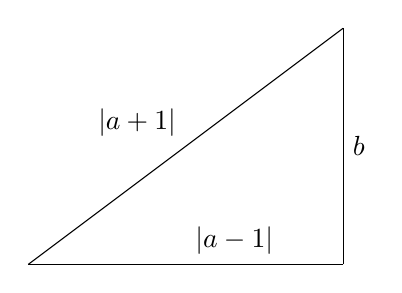
\begin{tikzpicture}
			\draw[black] (0,0) -- (4,0) node[midway, above right] {\(|a-1|\)};
			\draw[black] (4,0) -- (4,3) node[midway, right] {\(b\)};
			\draw[black] (0,0) -- (4,3) node[midway, above left] {\(|a+1|\)};
	\end{tikzpicture}\end{center}
	\begin{align*}
		b^2&=(a+1)^2-(a-1)^2\\
		&=4a
	\end{align*} also \(b=2\sqrt{a}\)
\end{proof}
\begin{Lemma}\label{Lem:KompQuad}
	Sei \(K\) ein Körper und \(K=K_0\subseteq K_1\dots\subseteq K_n\), \(K=L_0\subseteq L_1\dots\subseteq L_m\) Ketten quadratischer Körpererweiterungen.
	Dann ist \(K=L_0\subseteq \dots\subseteq L_m\subseteq K_1L_m\subseteq\dots \subseteq K_nL_m\) Kette höchstens quadratischer Körpererweiterungen.
\end{Lemma}
\begin{proof}
	Es ist \([K_iL_n:K_{i-1}L_n]\leq [K_i:K_{i-1}]=2\)
\end{proof}
\begin{Satz}
	Sei \(K\) ein Körper der Charakterisitik \(\neq 2\) und \(a\in\bar K\). Dann sind äquivalent:
	\begin{enumerate}
		\item Es gibt Kette quadratischer Erweiterungen \(K=K_0\subseteq \dots\subseteq K_n\) and \(a\in K_n\)
		\item Es gibt Galoiserweiterung \(L/K\) mit \(a\in L\) und \([L:K]=2^r\).
	\end{enumerate}
\end{Satz}
\begin{proof}
	Gelte \(1\) und sei \(K_n/K\) gegeben. Dann ist \(K_n/K\) ist separabel und nach \Cref{Satz:PrimElt} gilt \(K_n=K(b)\) für ein \(b\in K_n\). Sei \(L/K\) die normale Hülle von \(K_n/K\). Nach Konstruktion ist \(L/K\) der Zerfällungskörper vom Minimalpolynom \(f\) von \(b\). Seien \(b_1,\dots,b_n\) die Nullstellen von \(f\) in \(L\) mit \(b=b_1.\) Es ist \(L=K(b_1)\cdots K(B_n)\) Komposition. Da \(f\) das Minimalpolynom von \(b_i\) ist, ist \(K_n=K(b)=K(b_i)\) für alle \(i\) und somit ist \(K(b_i)/K\) durch Kette quadratischer Erweiterungen erreichbar. Nach \Cref{Lem:KompQuad} ist \(L\) als Kompositum durch quadratische Kette erreichbar. Gelte 2. und sei \(L/K\) Galoisch vom Grad \(2^r\). Dann ist \(G=\Gal(L/K)\) eine \(p\)-Gruppe für \(p=2\).
	\(G\) ist auflösbar somit gibt es nach \Cref{Kor:NormIndex} eine normale Untergruppe \(H\subseteq G\) mit \([G:H]=2\).
	Sei \(K_r=L\) und \(K_1=L^H\). Dann ist \([K_1:K_0]=2\) und \(K_r/K\) Galoisch von Grad \(2^{r-1}\). Also folgt die Aussage nach Induktion.
\end{proof}
\begin{Satz}
	\(\pi\in\RR\) ist transzendent über \(\QQ\).
\end{Satz}
\begin{Kor}
	\(\pi\not\in K(0,1)\) da \([\QQ(\pi):\QQ]=\infty\).
\end{Kor}
\begin{Kor}
	Wäre Winkeldrittelung immer möglich, so wäre \(\zeta_9\in K(0,1)\).
	\begin{center}\begin{tikzpicture}
			\coordinate (ME) at (-4,0);
			\coordinate (E) at (4,0);
			\coordinate (N) at (0,0);
			\coordinate (S) at (-0.5*4,0.866*4);
			\coordinate (Z) at (0.766*4, 0.642*4); 
			\draw (ME) -- (E);
			\draw[blue] (N) -- (S);
			\draw[blue] (ME) -- (S);
			\draw[blue] (ME) -- (N);
			\draw (N) -- (0,4);
			\draw[purple] (N) -- (Z);
			
			\pic [draw, "\( \)", angle radius=4cm, angle eccentricity=0.8] {angle = E--N--ME};
			\fill[purple] (Z) circle (2pt) node[above right] {\(\zeta_9\)};
			
	\end{tikzpicture}\end{center}
	Aber \([\QQ(\zeta_9):\QQ]=6\) ist keine Zweierpotenz also Widerspruch und die Aussage ist falsch.
\end{Kor}
\begin{Kor}[Würfelverdoppelung]
	Ist \(\sqrt[3]{2}\in K(0,1)\)? Es ist \[[\QQ(\sqrt[3]{2}):\QQ]=3\] keine Zweierpotenz, also nein.
	
\end{Kor}
\begin{Def}
	\begin{enumerate}
		\item[]
		\item Ein Körper \(L\) heißt quadratische abgeschlossen, wenn jedes quadratische Polynom in \(L[X]\) in \(L\) eine Nullstelle hat.
		\item Ein quadratischer Abschluss von \(K\) ist eine Erweiterung \(L/K\) sodass \(L\) quadratisch abgeschlossen ist und jede endliche Zwischenerweiterung \(L/L'/K\) lässt sich durch Kette quadratischer Erweiterungen erreichen.
	\end{enumerate}
\end{Def}
\begin{Bem}[Konstruktion eines quadratische Abschluss]
	Sei \[L=\set{a\in\bar K}{ K(a)/K \text{ ist durch Kette quadratischer Erweiterungen erreichbar }}.\]
	Wir haben gesehen: \(K(M)\) ist der quadratische Abschluss von \(\QQ(M\cup\bar M)\)
\end{Bem}
\subsection{Konstruktion des regulären \(n\)-Ecks}
Sei \(E\) die Menge der Ecken des regulären \(n\)-Ecks mit \(E\subseteq S^1=\set{z\in\CC}{ |z|=1}\). Es gilt \(E=\mu_n(\CC)\).
Sei \(\zeta_n\in\mu_n(\CC)\) primitiv. Ist \(\zeta_n\in K(0,1)\)?
Bekannt ist: \([Q(\zeta_n)/\QQ]\) ist Galoisch mit \(G=\Gal(\QQ(\zeta_n)/\QQ)=(\ZZ/n\ZZ)^*\) und \(|G|=\varphi(n)\).
Antwort: \[\zeta_n\in K(0,1)\iff \varphi(n)=2^r.\]
Wenn \(n=\prod_ip_i^{e_i}\) für verschiedene Primzahlen \(p_i\), dann ist \(\varphi(n)=\prod(p_i-1)p_i^{e_i-1}\). Das ist Zweierpotenz genau dann wenn \(e_i<2\) für \(p_i\neq 2\) und \(e_i=1\) nur wenn \(p_i-1\) eine Zweierpotenz ist.
\begin{Def}[Fermatsche Primzahl]
	Eine Fermatsche Primzahl ist eine Primzahl der Form \(p=2^m+1\).
\end{Def}
\begin{Bem}
	Wenn \(p\) prim dann ist \(\zeta_p\) konstruierbar \(\iff p\) ist Fermatsche Primzahl
\end{Bem}
\begin{Lemma}
	\(2^m+1\) prim \(\implies m=2^r\)
\end{Lemma}
\begin{proof}
	Sei \(m=qm'\) wobei \(q\) ungerade. Dann ist nach geometrischer Summe
	\[\dfrac{2^m+1}{2^{m'}+1}=\dfrac{1-(-2^{m'})^q}{1-(-2^{m'})}=\sum_{k=0}^{q-1}(-2^{m'})^k=\sum_{k=1}^q(-1)^{k+1}2^{m-km'}\] also \(2^{m}+1\) nicht prim.
\end{proof}
\begin{Bem}
	\(2^{2^r}+1\) ist prim für \(r=0,1,2,3,4\) aber für \(2^{2^5}+1=641\cdot 6700417\)
\end{Bem}
\begin{Bem}
	Fazit: Reguläre \(3,5,17\) Eck ist konstruierbar. Reguläre \(7,11,13,19\)-Eck nicht.
\end{Bem}
\begin{Bsp}
	Sei \(\alpha=\frac{2\pi}5\) und \(\beta=\frac{\pi-\alpha}2=\frac{3\pi}{16}\) und \(\gamma=2\beta=\frac 3 5\pi\)
	\begin{center}\begin{tikzpicture}
			\coordinate (E1) at (4*0.951,4*0.309);
			\coordinate (E2) at (4*0,4*1);
			\coordinate (E3) at (-4*0.951,4*0.309);
			\coordinate (E4) at (-4*0.588,-4*0.809);
			\coordinate (E5) at (4*0.588, -4*0.809);
			\coordinate (N) at (0,0);
			\draw[name path=K1] (E1) -- (E2);
			\draw[name path=K2] (E2) -- (E3);
			\draw[name path=K3] (E3) -- (E4);
			\draw[name path=K4] (E4) -- (E5);
			\draw[name path=K5] (E5) -- (E1);
			\draw[red] (0,0) -- (E2);
			\draw[red] (0,0) -- (E3);
			\pic [draw, "\(\gamma\)", angle radius=1cm, angle eccentricity=0.5] {angle = E1--E5--E4};
			\pic [draw, "\(\alpha\)", angle radius=1cm, angle eccentricity=0.5] {angle = E2--N--E3};
			\pic [draw, "\(\beta\)", angle radius=1cm, angle eccentricity=0.5] {angle = E3--E2--N};
			\pic [draw, "\(\beta\)", angle radius=1cm, angle eccentricity=0.5] {angle = N--E3--E2};
			
			
	\end{tikzpicture}\end{center}
	Sei weiter \(\delta=\frac{\pi-\gamma}2\).
	Dann ist \(\delta=\frac{1}{5}\pi\) und \(\gamma-2\delta=\frac 1 5\pi=\delta\)
	\begin{center}\begin{tikzpicture}
			\coordinate (E1) at (4*0.951,4*0.309);
			\coordinate (E2) at (4*0,4*1);
			\coordinate (E3) at (-4*0.951,4*0.309);
			\coordinate (E4) at (-4*0.588,-4*0.809);
			\coordinate (E5) at (4*0.588, -4*0.809);
			\coordinate (N) at (0,0);
			\coordinate (F) at (1.454,-0.473);
			\draw[name path=K1] (E1) -- (E2) node[midway,above]{\(1\)};
			\draw[name path=K2] (E2) -- (E3) node[midway,above]{\(1\)};
			\draw[name path=K3] (E3) -- (E4) node[midway, below left]{\(1\)};
			\draw[name path=K4] (E4) -- (E5);
			\draw[name path=K5] (E5) -- (E1);
			\draw[name path=D,red] (E2) -- (E4) node[midway, above left] {\(d\)};
			\draw[name path=EO,red] (E2) -- (F) node[pos=0.6, below left] {\(1\)};
			\draw[name path=EU,red] (E5) -- (F) node[pos=0.6, below left] {\(e\)};
			\draw[blue] (E1) -- (F);
			\pic [draw, "\(\delta\)", angle radius=1cm, angle eccentricity=0.65] {angle = E3--E2--E4};
			\pic [draw, "\(\delta\)", angle radius=1cm, angle eccentricity=0.65] {angle = E4--E2--E5};
			\pic [draw, "\(\delta\)", angle radius=1cm, angle eccentricity=0.65] {angle = E5--E2--E1};
			\pic [draw, "\(2\delta\)", angle radius=1cm, angle eccentricity=0.65] {angle = E5--E4--E2};
			\pic [draw, "\(2\delta\)", angle radius=1cm, angle eccentricity=0.65] {angle = E2--E5--E4};
			\pic [draw, "\(\delta\)", angle radius=1cm, angle eccentricity=0.65] {angle = E1--E5--E2};
			\pic [draw, "\(3\delta\)", angle radius=1cm, angle eccentricity=0.65] {angle = E5--F--E1};
			\pic [draw, "\(2\delta\)", angle radius=1cm, angle eccentricity=0.65] {angle = E1--F--E2};
			\pic [draw, "\(2\delta\)", angle radius=1cm, angle eccentricity=0.65] {angle = E2--E1--F};
			\pic [draw, "\(\delta\)", angle radius=1cm, angle eccentricity=0.65] {angle = F--E1--E5};
			\fill[green] (-2.5,0.7) circle (0pt) node[above] {\(A\)};
			\fill[green] (0,-0.7) circle (0pt) node[above] {\(B\)};
			\fill[green] (2.8,-1) circle (0pt) node[above] {\(C\)};
			\fill[green] (1.6,1.6) circle (0pt) node[above] {\(D\)};
			
			
	\end{tikzpicture}\end{center}
	Die Dreiecke \(A\) und \(C\) sind ähnlich und die Dreiecke \(B\) und \(D\) sind ähnlich, da sie gleiche Winkel haben.
	Sei \(d\) die Länge der Diagonalen und \(e=d-1\)
	Es gilt also \(\frac 1 d=\frac{1}{e}=\frac{1}{d-1}\)
	Also ist \(d^2-d=1\) was \(d=\dfrac{\sqrt 5+1}{2}\) impliziert.
	Konstruiere also
	\begin{center}\begin{tikzpicture}
			\coordinate (N) at (0,0);
			\coordinate (E) at (4,0);
			\coordinate (F) at (4,2);
			\draw (N) -- (E) node[midway, below]{\(1\)};
			\draw (E) -- (F) node[midway, right]{\(\frac 1 2\)};
			\draw (N) -- (F) node[midway, above]{\(\frac{\sqrt 5}{2}\)};
	\end{tikzpicture}\end{center}
	und dann konstruiere 5-Eck.
\end{Bsp}
\section{Auflösbarkeit durch Radikale}
\begin{Def}
	Sei \(K\) ein Körper der Charakteristik 0.
	\begin{enumerate}
		\item Eine einfache Radikalerweiterung ist eine Körpererweiterung \(L/K\) sodass \(L=K(a)\) für ein \(a\) mit \(a^n\in K\) für ein \(n\in\NN_1\)
		\item \(L/K\) heißt Radikalerweiterung, wenn es eine Kette \(K=K_0\subseteq\dots \subseteq K_r=L\) gibt sodass \(K_i/K_{i-1}\) eine einfache Radikalerweiterung ist.
		\item \(L/K\) ist auflösbar durch Radikale, wenn es für jedes \(a\in L\) eine Radikalerweiterung \(L'/K\) und Einbettung \(K(a)\subseteq L'\) existiert.
	\end{enumerate}
\end{Def}
\begin{Bem}
	Wenn \(L/K\) endlich, dann ist \(L=K(a)\) für ein \(a\in L\).
	Dann
	\[L/K \text{ ist auflösbar durch Radikale}\iff L\text{ ist in einer Radikalerweiterung enthalten}\]
\end{Bem}
\begin{Bem}
	Notation: Wenn \(L/K\) einfache Radikalerweiterung, \(L=K(a)\) und \(a\) Nullstelle von \(X^n-b\) könnte schreiben \(a=\sqrt[n]{b}\) aber das ist ungenau da \(X^n-b\) \(n\) verschiedene Nullstellen hat.
\end{Bem}
\begin{Bsp}
	Sei \(f=X^3-2\) und sei \(a=\sqrt[3]{2}\in\RR\). Wenn \(K=\QQ(a)\) dann ist \([K(a):K]=1\) aber \([K(\zeta_3 a):K]=2\)
\end{Bsp}
\begin{Bem}
	Angenommen \(K\) ist ein Körper von Charakteristik \(\neq n\) und \(\mu_n(\bar K)\subseteq K\) Dann sei \(\zeta_n\in\mu_n(\bar K)\) primitiv.
	Die Nullstellen von \(f=X^n-b\) sind \(a,\zeta_na,\zeta_n^2a,\dots,\zeta_n^{n-1}a\) also 
	\(X^n-b=\prod\limits_{k=0}^{n-1}(X-\zeta_n^ka)\) und \(K(a)=K(\zeta_n^ka)\) für jedes \(k\) da \(K\) \(\zeta_n\) enthält. In diesem Fall ist die Bezeichnung \(K(\sqrt[n]{b})=K(a)\) für irgendein \(a\) mit \(a^n=b\). Das ist ein Zerfallskörper von \(X^n-b\).
\end{Bem}
\begin{Lemma}\label{Lem:EinfRadZykl}
	Sei \(K\) ein Körper der Charakteristik \(\neq n\) und \(\mu_n(\bar K)\subseteq K\). Dann gibt es einen injektiven Gruppenhomomorphismus \(\Gal(K(\sqrt[n]{a})/K)\to \mu_n(K)\cong \ZZ/n\ZZ\). Insbesondere ist \(G=\Gal(L/K)\) zyklisch.
\end{Lemma}
\begin{proof}
	Sei \(\sigma\in G\) und \(b=\sqrt[n]{a}\). Es ist \(\sigma(b)\) ist eine Nullstelle von \(X^n-a\) also ist \(\sigma(b)=\zeta b\) für ein \(\zeta\in\mu_n(K)\).
	Da \(\mu_n(\bar K)\subseteq K\) ist für \(\zeta'\in\mu_n(\bar K):\)
	\[\sigma(\zeta'b)=\zeta'\sigma(b)=\zeta'\zeta b.\]
	Sei \(\psi\colon G\to \mu_n(\bar K), \ \psi(\sigma)=\frac{\sigma(b)}{b}\). Eine Rechnung zeigt, dass das ein Gruppenhomomorphismus ist. Angenommen \(\psi(\sigma)=1\).
	Dann ist \(\sigma=\id\) auf Menge der Nullstellen und da \(K(\sqrt[n]{a})/K\) Zerfällungskörper ist, ist \(\sigma=\id\).
\end{proof}
\begin{Def}
	Sei \(E\) eine Eigenschaft von Gruppen (z.B. zyklisch, auflösbar, abelsch...) Eine Körpererweiterung \(L/K\) hat die Eigenschaft \(E\), wenn \(L/K\) Galoisch ist und \(\Gal(L/K)\) diese Eigenschaft \(E\) hat.
\end{Def}
\begin{Satz}\label{Satz:ZyklWurzel}
	Sei \(Char(K)\neq n\) und \(\mu_n(\bar K)\subseteq K\). Wenn \(L/K\) zyklisch von Grad \(n\), dann ist \(L=K(\sqrt[n]{a})\) für ein \(a\in K\).
\end{Satz}
\begin{proof}
	Sei \(\sigma\in\Gal(L/K)\) ein Erzeuger. Als Endormorphismus gilt \(\sigma^n-\id=0\). Sei \(\mu_\sigma\) Minimalpolynom von \(\sigma\).
	Dann gilt \(\mu_\sigma\mid X^n-1=\prod_{\zeta\in\mu_n}(X-\zeta)\). Somit ist \(\sigma\) diagonalisierbar und die Eigenwerte sind die Nullstellen von \(\mu_\sigma\). Sei \(B\subseteq \mu_n\) die Menge dieser Nullstellen. Für \(\zeta\in \mu_n(\bar K)\) sei \(V_\zeta=\set{x\in L}{ \sigma(x)=\zeta x}\). Es gilt \(V_\zeta\neq 0\iff \zeta\in B\) und
	\(L=\oplus_{\zeta\in\mu_n}V_\zeta\).
	Sei \(x\in V_\zeta\) mit \(x\neq 0\). Dann gilt \(x^{-1}\in V_{\zeta^{-1}}\) und somit haben wir inverse Abbildungen 
	\[V_{\zeta'}\stackrel{x}\to V_{\zeta\zeta'}\stackrel{x^{-1}}\to V_{\zeta'}\] somit ist \(V_{\zeta'}\cong V_{\zeta\zeta'}\)
	Das zeigt: \(B\subseteq \mu_n(\bar K)\) ist Untergruppe und wenn \(\zeta\in B\) Erzeuger ist, dann  ist \(V_1\cong V_\zeta\cong V_{\zeta^2}\cong\dots\).
	Also ist \[\dim(V_{\zeta^i})=\dim(V_1)\] und \(\dim(V_1)=[\mu_n:B]\) denn \(n=\dim(L)=|B|\cdot \dim(V_1)\).
	Es ist 
	\[V_1=\set{x\in L}{ \sigma(x)=x}=L^{\langle \sigma\rangle}=L^G=K\] also \(\dim(V_1)=1\) und somit \(\mu_n=B\) und \(\dim(V_\zeta)=1\) für alle \(\zeta\in\mu_n\).
	Sei \(\zeta_n\in\mu_n\) primitiv. Wähle \(b\in V_{\zeta_n}\) mit \(b\neq 0\). Es ist \(\langle b^i\rangle=V_{\zeta_n^i}\) somit erzeugen \(1,b,\dots, b^{n-1}\) den \(K\)-Vektorraum \(L\). Also ist \(L=K(b)\).
	Es ist \(\sigma(b)=\zeta_nb\) also \(\sigma(b^n)=b^n\) und somit ist \(a=b^n\in L^G=K\). Das zeigt: \(b\) ist Nullstelle von \(X^n-a\in K[X]\)
\end{proof}
\begin{Lemma}
	Die Komposition von Radikalerweiterungen ist eine Radikalerweiterung.
\end{Lemma}\label{Lem:KompRad}
\begin{proof}
	Seien \(K=K_0\subseteq K_1\subseteq \dots \subseteq K_r\) und \(K=L_0\subseteq L_2\subseteq \dots \subseteq L_n\) Ketten von einfachen Radikalerweiterungen.
	Dann ist \(K=K_0\subseteq \dots K_r=K_rL_0\subseteq K_rL_1\subseteq\dots \subseteq K_rL_n\) Kette von einfachen Radikalerweiterungen, denn wenn \(L_i=L_{i-1}(a_i)\) mit \(a_i^n\in L_{i-1}\) dann ist \(K_rL_i=K_rL_{i-1}(a_i)\) und \(a_i^n\in K_rL_{i-1}\)
\end{proof}
\begin{Lemma}\label{Lem:AuflRad}
	Sei \(L/K\) eine endliche Körpererweiterung in Charakterisitk \(0\).
	\begin{enumerate}
		\item \(L/K\) ist Radikalerweiterung \(\implies \) normale Hülle von \(L/K\) ist Radikalerweiterung.
		\item \(L/K\) ist auflösbar durch Radikale \(\iff\) normale Hülle von \(L/K\) ist auflösbar durch Radikale.
	\end{enumerate}
\end{Lemma}
\begin{proof}
	1):Sei \(L=K(a)\) und seien \(a=a_1,\dots,a_r\in\bar K\) die Nullstellen vom Minimalpolynom von \(a\). Also ist die normale Hülle gegeben durch \(M=K(a_1)\cdots K(a_r)\).
	Es ist \(K(a_i)\cong K(a)\) Radikalerweiterung über \(K\). Nach \Cref{Lem:KompRad} ist also \(M/K\) eine Radikalerweiterung.\\
	2): Sei \(L=K(a_1)/K\) auflösbar durch Radikale, dh. es gibt \(L'/L\) sodass \(L'/K\) Radikalerweiterung ist. Sei \(M/K\) bzw \(M'/K\) die normale Hülle von \(L/K\) bzw \(L'/K\). Dann ist \(M\subseteq M'\). Nach 1) ist \(M'/K\) Radikalerweiterung also \(M/K\) auflösbar durch Radikale.
	Sei andersrum \(M/K\) die normale Hülle von \(L/K\) und \(M/K\) auflösbar durch Radikale, dh. Es gibt \(M'/M\) sodass \(M'/K\) Radikalerweiterung. Dann ist \(L/K\) auflösbar durch Radikale nach Definition.
\end{proof}
\begin{Satz}
	Sei \(L/K\) endliche Körpererweiterung in Charakteristik \(0\) und \(M/K\) eine normale Hülle. Dann ist \(L/K\) auflösbar durch Radikale \(\iff L/K\) auflösbar.
\end{Satz}
\begin{proof}
	Nach \Cref{Lem:AuflRad} ist ohne Einschränkung \(L/K\) Galoisch.
	Sei \(n=[L:K]\) und \(K'=K(\mu_n)\) und \(L'=L(\mu_n)\).
	Da \(L/K\) Galoisch ist \(L'/K'\) Galoisch und \(L'/K\) Galoisch. Es sind \(\Gal(K'/K)\) und \(\Gal(L'/L)\) abelsch, insbesondere auflösbar.
	Es ist \[\Gal(L/K)\cong \Gal(L'/K)/\Gal(L'/L)\] und \(\Gal(L'/K)/\Gal(L'/K')\cong \Gal(K'/K)\).
	Also ist \begin{align*}
		\Gal(L/K)\text{ auflösbar }&\iff \Gal(L'/K) \text{ auflösbar}\\
		&\iff \Gal(L'/K') \text{ auflösbar}
	\end{align*}
	und \(K'/K\) und \(L'/L\) sind Radikalerweiterungen. Somit ist \(L/K\) auflösbar durch Radikale \(\iff L'/K'\) auflösbar durch Radikale. Somit ist ohne Einschränkung \(L=L'\) und \(K=K'\).
	Sei \(L/K\) auflösbar. Wähle Normalreihe in \(\Gal(L/K)\) mit primzyklischen Quotienten. Das entsprich \(K=K_0\subseteq K_1\subseteq\dots\subseteq K_n=L\) mit \(K_i/K_{i-1}\) Galoisch und \(\Gal(K_i/K_{i-1})\cong \ZZ/p_i\ZZ\).  \Cref{Satz:ZyklWurzel} impliziert, dass \(K_i/K_{i-1}\) eine einfache Radikalerweiterung ist. Somit ist \(L/K\) eine Radikalerweiterung. Insbesondere ist \(L/K\) auflösbar durch Radikale.\\
	Sei andersrum \(L/K\) auflösbar durch Radikale. Es gibt \(L'/L\), sodass \(L'/K\) Radikalerweiterung ist. Ohne Einschränkung ist \(L'/K\) Galoisch. Es gibt Kette \(K=K_0\subseteq K_1\subseteq\dots\subseteq K_n=L'\) sodass \(K_i/K_{i-1}\) einfache Radikalerweiterung ist.
	Behauptung: \(\Gal(L'/K)\) ist auflösbar. Dann ist \(\Gal(L/K)\) als Quotient von \(\Gal(L'/K)\) auch auflösbar.
	\Cref{Lem:EinfRadZykl} impliziert, dass \(K_i/K_{i-1}\) Galoisch ist mit zyklischer Galoisgruppe. DIe Körperkette entspricht Kette von Untergruppen in \(\Gal(L'/K)\). Das ist eine abelsche Normalreihe.
\end{proof}
\begin{Kor}
	Jede Gleichung von Grad \(\leq 4\) in Charakterisitk \(0\) ist durch Radikale auflösbar, dh. \(f\in K[X]\) mit \(\deg(f)\leq 4\) und \(L/K\) Zerfällungskörper von \(f\), dann ist \(G=\Gal(L/K)\) auflösbar.
\end{Kor}
\begin{proof}
	Haben injektiven Gruppenhomomorphismus \(G\to S_4\). Da \(S_4\) auflösbar ist, ist \(G\) auflösbar.
\end{proof}
\begin{Satz}
	Für jede endliche Gruppe \(G\) gibt es eine Galoiserweiterung \(L/K\) in Charakteristik \(0\) mit \(G=\Gal(L/K)\).
\end{Satz}
\begin{proof}
	Wähle \(G\to S_n\) injektiv mit \(|n|=G\). Wenn \(L/K'\) existiert mit \(\Gal(L/K')=S_n\) dann gilt für \(K=L^G\) dass \(\Gal(L/K)=G\) ist.
	\(S_n\) operiert auf \(L=\QQ(X_1,\dots,X_n)\) durch Permutation der Variablen. Das gibt Homomorphismus \(S_n\to\Aut(L)\) der injektiv ist. Der Körper \(K=L^{S_n}\) gibt \(\Gal(L/K)=S_n\).
\end{proof}
\begin{Bem}
	\(S_5\) ist nicht auflösbar. 
\end{Bem}
\begin{Bem}
	\begin{enumerate}
		\item[]
		\item Es gibt eine Definition von Auflösbar durch Radikale in beliebiger Charakteristik, für die der letzte Satz gilt
		\item Frage: Wenn \(K\) gegeben, welche Gruppen \(G\) sind als Galoisgruppen über \(K\) realisierbar, dh. gibt es \(L/K\) Galoisch mit \(\Gal(L/K)=G\).
		\begin{enumerate}
			\item \(K=\RR\) Dann ist \(G=\Set{1}\) und \(G=\ZZ/2\ZZ\) möglich.
			\item Wenn \(K\) endlich ist: Genau die zyklischen Gruppen sind möglich, denn \[\Gal(\FF_{q^n}/\FF_q)\cong\langle Fr\rangle\cong\ZZ/n\ZZ.\]
			\item \(K=\QQ\) Frage ist offen. \(G=S_p\) nach Übungsaufgabe?
			\(G=S_n\) möglich (Hilbert).
		\end{enumerate}
	\end{enumerate}
\end{Bem}
\begin{Satz}
	Es gibt Gleichungen vom Grad \(5\) die nicht auflösbar sind
\end{Satz}
\begin{proof}
	\(S_5\) ist Galoisgruppe von \(M/\QQ\) für ein \(M/\QQ\) Galoisch. Es ist \(H=S_4=\Stab(1)\subseteq S_5\) also \([G:H]=5\) und somit \([M^H:K]=5\). Es ist \(M=K(a)\) für ein \(a\). Die normale Hülle von \(M^H/K\) entspricht nach Galoiskorrespondenz \(\bigcap_{g\in S_5}gHg^{-1}=\Set{e}\), also ist \(M/K\) die normale Hülle von \(M^H=\QQ(a)=\QQ[X]/(f)\) wobei \(f\) das Minimalpolynom von \(a\) ist. Damit ist \(S_5\) Galoisgruppe von \(f\) und \(S_5\) ist nicht auflösbar. Es ist \(\deg(f)=[\QQ(a):\QQ]=5\)
\end{proof}